	\documentclass[]{article}
	\usepackage{tikz}  %TikZ central library is called.
\usetikzlibrary{positioning,shapes,fit,arrows}
\tikzset{set/.style={draw,circle,inner sep=0pt,align=center}}
\usepackage{amssymb} 

%opening
\title{Algebra}
\author{José Guilherme Vanz}

\begin{document}

\maketitle

\section{Numbers}

\subsection{Natural numbers $\mathbb{N}$}

\textit{Natural numbers} ($\mathbb{N}$) start from 1 and goes forever always increasing by 1.

\[ 1,2,3,4,5... 1000, 1000000, ..., \infty\]

Negatives numbers, numbers with decimals, zero are \textbf{not} Natural numbers. For example:

\[ -1,000 \]
\[\frac{1}{3}\]
\[ 89.1 \]

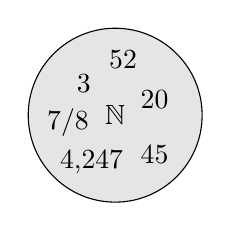
\begin{tikzpicture}
\node[set,fill=gray!20,text width=2.2cm] (nat) at (0,0) {$\mathbb{N}$};
\node[draw=none] at (0.5,0.2) {20};
\node[draw=none] at (0.5,-0.5) {45};
\node[draw=none] at (-0.4,0.4) {3};
\node[draw=none] at (0.1,0.7) {52};
\node[draw=none] at (-0.6,-0.1) {7/8};
\node[draw=none] at (-0.3,-0.6) {4,247};
\end{tikzpicture}

\subsection{Integers $\mathbb{Z}$}

All number from -$ \infty $ to $ \infty $. They can be written without any fractions or decimals

\[-4, -3, -2, -1, 0, 1, 2, 3, 4\]

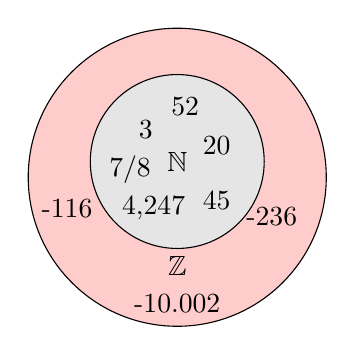
\begin{tikzpicture}

\node[set,fill=red!20,text width=3.8cm,label={[below=79pt of int]$\mathbb{Z}$}] (int) at (0,-0.2)  {};
\node[draw=none] at (-1.4,-0.6) {-116};
\node[draw=none] at (0,-1.8) {-10.002};
\node[draw=none] at (1.2,-0.7) {-236};
\node[set,fill=gray!20,text width=2.2cm] (nat) at (0,0) {$\mathbb{N}$};
\node[draw=none] at (0.5,0.2) {20};
\node[draw=none] at (0.5,-0.5) {45};
\node[draw=none] at (-0.4,0.4) {3};
\node[draw=none] at (0.1,0.7) {52};
\node[draw=none] at (-0.6,-0.1) {7/8};
\node[draw=none] at (-0.3,-0.6) {4,247};
\end{tikzpicture}



\subsection{Rational Numbers $\mathbb{R}$}

A rational number ($\mathbb{R}$) is a number that can be written as:

\[ \frac{a}{b} \]

where $a$ and $b$ are \textit{integers} and $b$ is different of zero $ b \neq 0$

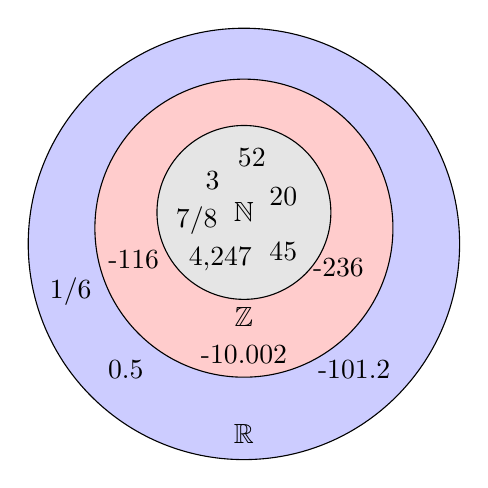
\begin{tikzpicture}
\node[set,fill=blue!20,text width=5.5cm,label={[below=140pt of rea]$\mathbb{R}$}] 
(nat) at (0,-0.4)  (rea) {};
\node[draw=none] at (-1.5,-2) {0.5};
\node[draw=none] at (1.4,-2) {-101.2};
\node[draw=none] at (-2.2,-1) {1/6};

\node[set,fill=red!20,text width=3.8cm,label={[below=79pt of int]$\mathbb{Z}$}] (int) at (0,-0.2)  {};
\node[draw=none] at (-1.4,-0.6) {-116};
\node[draw=none] at (0,-1.8) {-10.002};
\node[draw=none] at (1.2,-0.7) {-236};
\node[set,fill=gray!20,text width=2.2cm] (nat) at (0,0) {$\mathbb{N}$};
\node[draw=none] at (0.5,0.2) {20};
\node[draw=none] at (0.5,-0.5) {45};
\node[draw=none] at (-0.4,0.4) {3};
\node[draw=none] at (0.1,0.7) {52};
\node[draw=none] at (-0.6,-0.1) {7/8};
\node[draw=none] at (-0.3,-0.6) {4,247};
\end{tikzpicture}

\subsection{Fraction to decimals}

\[ \frac{7}{16} = 0.4375 \] <--- terminating

\[ \frac{1}{3} = 0.\bar{3} = 0.33333... \] <--- repeating 

% I'm not sure if this subsection should be here. But I'll keep it for now
\subsection{Ratio}
In Math a ratio between two numbers indicates how many times the first number contains the seconds. 

\subsection{Irrational Numbers}

Cannot be written as ratios of integers

\begin{tikzpicture}
\node[set,fill=gray!20,text width=3cm] (irr) at (0,0) {};
\node[draw=none] at (0,0.3) {e$\approx$2.71828182845};
\node[draw=none] at (0,-0.3) {\pi$\approx$3.141592653589};

\end{tikzpicture}

\subsection{Real Numbers}

\begin{tikzpicture}
 \draw (0,0) ellipse (7cm and 4cm);
\node[draw=none] at (0,3.5) {Real numbers}; 
\node[set,fill=blue!20,text width=5.5cm,label={[below=140pt of rea]$\mathbb{R}$}] 
(nat) at (0,-0.4)  (rea) {};
\node[draw=none] at (-1.5,-2) {0.5};
\node[draw=none] at (1.4,-2) {-101.2};
\node[draw=none] at (-2.2,-1) {1/6};

\node[set,fill=red!20,text width=3.8cm,label={[below=79pt of int]$\mathbb{Z}$}] (int) at (0,-0.2)  {};
\node[draw=none] at (-1.4,-0.6) {-116};
\node[draw=none] at (0,-1.8) {-10.002};
\node[draw=none] at (1.2,-0.7) {-236};
\node[set,fill=gray!20,text width=2.2cm] (nat) at (0,0) {$\mathbb{N}$};
\node[draw=none] at (0.5,0.2) {20};
\node[draw=none] at (0.5,-0.5) {45};
\node[draw=none] at (-0.4,0.4) {3};
\node[draw=none] at (0.1,0.7) {52};
\node[draw=none] at (-0.6,-0.1) {7/8};
\node[draw=none] at (-0.3,-0.6) {4,247};

\node[set,fill=gray!20,text width=3cm] (irr) at (5,0) {Irrational numbers};
\node[draw=none] at (5,0.4) {e$\approx$2.71828182845};
\node[draw=none] at (5,-0.4) {\pi$\approx$3.141592653589};

\end{tikzpicture}

\subsection{Set}

A \textbf{set} is a collection of numbers
A \textbf{subset} is a set of numbers that are all contained in another set

\end{document}
